\documentclass[12pt]{article}
\usepackage[margin=1in]{geometry} 
\usepackage{amsmath, amssymb, amsthm}
\usepackage{tcolorbox}
\usepackage{lastpage}
\usepackage{fancyhdr, accents}
\usepackage{natbib}
\usepackage{graphicx}

\pagestyle{fancy}
\setlength{\headheight}{40pt}
\graphicspath{ {sources/} }

\newenvironment{solution}
  {\renewcommand\qedsymbol{$\blacksquare$}
  \begin{proof}[Solution]}
  {\end{proof}}
\renewcommand\qedsymbol{$\blacksquare$}

\newcommand{\ubar}[1]{\underaccent{\bar}{#1}}

\newcommand\tab[1][1cm]{\hspace*{#1}}

\title{CSC110Y1-F Fall 2020 - Fundamentals of Computer Science 1 \\ Course Project Proposal}
\author{
  Ching Chang\\
  \and
  Letian Cheng\\
  \and
  Arkaprava Choudhury\\
  \and
  Hanrui Fan
}
\date{\today}

\begin{document}

\maketitle
% Make cover page. Not to be submitted, but for aesthetic.

\newpage

\lhead{Ching Chang, Letian Cheng \\ Arkaprava Choudhury, Hanrui Fan} 
\rhead{CSC110Y1-F Fall 2020 \\ Fundamentals of Computer Science 1 \\ Course Project Proposal} 
\cfoot{\thepage\ of \pageref{LastPage}}

\begin{enumerate}
\item \section*{Part 1}

There are 2 main types of citations: text \citet{But20} and Parenthetical \citep{Bra20}.

command citet \citet{Mar20} is the same as \cite{Mel93}.


\bibliography{references}
\bibliographystyle{apalike}

\begin{solution}

\end{solution}

\newpage

\item \section*{Part 2}

\begin{itemize}
  \item Give an overview of any background knowledge necessary for the reader to understand the problem you are studying.
  \item Provide context for the problem and motivate why you have chosen your research question.
  \item Your research question should be in \emph{bold}; it should be fairly concise, but can be more than one sentence.
\end{itemize}

\begin{solution}

\end{solution}

\newpage

\item \section*{Part 3}

\begin{itemize}
    \item State the source (e.g., government/organization website) and format (e.g., text, csv, json, image) of the dataset, and give some sample data contained inside that dataset.
    \item Don’t be afraid to cobble together your own dataset, such as creating a collection of images that are related. Or to combine two datasets from different sources.
    \item You will also submit a small sample of your dataset to MarkUs along with your project proposal document. (See more below)
\end{itemize}


The data we show here is based on joint estimates by Brazilian National Institute of Space Research and the United Nations Food and Agriculture Organization with map data provided by MapBiomas.\\
    The data is presented as a text-based table, but we will convert it into a csv file. The data shows the area of the Amazon rainforest in Brazil, which accounts for about 60\% of the total area of the country.\\
    For these data we did some pre-processing, we first removed items in the data that had NA (unrecorded or incomplete data), these included data up to 1985 and 2019, but we needed to record data from pre-1970 as this is the baseline data for the subsequent percentage change.\\
    We then selected data from the start of 1988 because our team considered the absence of the change in deforestation loss data between 1978-1987 to be unrepresentative, so we filtered the 1978-1987 data as well.\\
    At the same time, these data contain four columns including estimated remaining forest cover, average annual forest area loss, percentage of forest cover compared to 1970 area, and total forest area lost since 1970.\\
    
\begin{itemize}
  \item 
  {
    CO2 data.  https://ourworldindata.org/grapher/annual-co-emissions-by-region

    \begin{tabular}{ |c|c|c| }
    \hline
    Entity & Year & Annual CO2 emissions \\
    \hline
      South America & 2010 & 1059.075401726349 \\
      \hline
      South America & 2011 & 1062.6963727613836 \\
      \hline
      South America & 2012 & 1125.3927407850085 \\
      \hline
      South America & 2013 & 1166.250041134838 \\
      \hline
      South America & 2014 & 1198.3039835470736 \\
      \hline
      South America & 2015 & 1170.890808102911 \\
      \hline
      South America & 2016 & 1134.3849989543753 \\
      \hline
      South America & 2017 & 1125.5205007738507 \\
      \hline
      South America & 2018 & 1112.9340357582964 \\
      \hline
    \end{tabular}
 
  }
  \item
  {
    precipitation data. https://neo.sci.gsfc.nasa.gov/view.php?datasetId=TRMM\_3B43M

    This is the Global rainfall map in August, 2016. We can extract the exact numbers using colour table provided.

    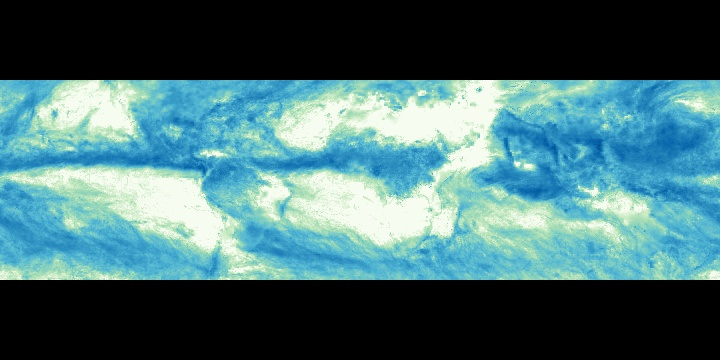
\includegraphics[scale = 0.6]{Global-rainfall-Aug2016.png}

    here is the colour table: 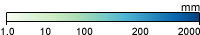
\includegraphics{Global-rainfall-Aug2016-table.png}
  }
  \item
  {
    Deforestation data. https://rainforests.mongabay.com/amazon/deforestation\_calculations.html

    \begin{tabular}{ |c|c|c|c|c|c| }
    \hline
    Period &	Estimated Natural Forest Cover &	Deforestation (INPE) \\
      \hline
      2015 & 3,413,662  & 6,207  \\
      \hline
      2016 & 3,406,796  & 7,893 \\
      \hline
      2017 & 3,399,308  & 6,947 \\
      \hline
      2018 & 3,390,835  & 7,900 \\
      \hline
    \end{tabular}
 
  }
\end{itemize}

\textbf{\large 4. A computational plan for your project. (300–500 words)}
\begin{solution}
\end{solution}

\newpage

\item \section*{Part 4}

\begin{itemize}
    \item Describe the kinds of computations you plan to perform, such as: data transformation/filtering/aggregation, computational models, and/or algorithms.
    \item Explain how your program will report the results of your computation in a visual and/or interactive way. You don’t need to go into a lot of details here, but it should be clear what you plan to do.
\end{itemize}

\textbf{Technical requirement:} for your project, you must use at least one Python library/module that we have not covered in this course, \emph{or} use \underline{plotly} or \underline{pygame} to a much larger extent than what what have given you so far in this course. (See examples and note in the next section).

\begin{itemize}
    \item In this part of your proposal, you should also describe one new library you intend to use, how you will use it, and why it is appropriate. Refer to specific functions, data types, and/or capabilities of the library that make it relevant for solving the problem you wish to solve.
\end{itemize}

\begin{solution}\

We first create a function that parses the \texttt{html} element of the stats on the website as a string, and converts it to a \texttt{nested array} so that it’s easier to work with. This will involve using a \texttt{for loop}, \texttt{if statements}, and an \texttt{accumulator} keeping track of the data parsed so far. Using this function, we will collect our data for deforestation in the Amazon rain-forest over the past few decades. With the data now converted into a form that we can easily manipulate, we shall focus on analysing the data using our own functions.

For this project, we use smooth polynomial fitting to relate two of the variables in our \texttt{nested list}. Now, although there exist readily available functions that would do the same in the module scipy, we try implementing our own functions for the same, to test our learning from the course.

We split the mathematical algorithm for this problem using top-down design. Firstly, the main function would have two lists, \texttt{l\_x, l\_y}, of same length as input (for the two variables), along with an integer $n$ (where $n \leq \texttt{len(l\_x)}$; representing degree of intended polynomial). The function body would have calls to helper functions. Note: this is only a rough outline and the exact technical details may be changed based on the results after testing the functions.

Firstly, we have a function to calculate the perpendicular distance of one point from a given polynomial. As opposed to the naive approach to the problem, we use Newton-Raphson method \textit{repeatedly} to estimate a solution for the derivative of the expression for the difference between the point and the polynomial, hence finding the coordinates of the foot of perpendicular, and consequently, the length of perpendicular.

The first estimate for the polynomial will be trivial, and we will then run the simplex algorithm to minimize the sum of the squares of the perpendiculars using two more helper functions, yielding the polynomial regression model. We now move towards plotting the resulting graph using the matplotlib library.

We also plan to write a function to calculate the coefficient of determination to check whether the graph shows an appropriate relationship between the independent variable (forest cover) and the dependent variable. 

In addition to the graph, we plan to create an interactive text-based report of our data, where the user  inputs a value for the independent or dependent variable, and the program will provide the corresponding dependent or independent value, coefficient of determination, or the slope of the tangent at the point, depending on which one the user asks for. The output will be text-based, and will require string concatenation, and if statements to check whether to add trivial information to the report. 

The input/output model will use while loops and input prompts to keep the program interactive. We also extrapolate the data to yield the predictions about future data using the interactive i/o model. Finally, we use the extrapolated data to summarize the upcoming significant years where the dependent variable will reach a certain milestone.


\end{solution}

\maketitle

\newpage

 \end{enumerate}


\end{document}

